\documentclass[12pt,a4paper]{article}
\usepackage{preamble}
\usepackage{graphicx}
\usepackage[bottom]{footmisc}
\usepackage{array}
\usepackage{tikz}
\usepackage{calc}
\newcommand\sessiontitle{Lab Session 4}
\newcommand\sessionsubtitle{Edge detection: Derivative operators}

\newcommand\laminus{\makebox[\widthof{+}][r]{-}} %% left-aligned minus of the width of a "+"

%%%%%%%%%%%%%%%%%%%%%%%%%%%%%%%%%%%%%%%%%%
\begin{document}

\paragraph{Preparation.} Enter the Conda environment and open the notebook \texttt{task4.ipynb}. Enter the ``\texttt{\%pylab}'' and ``\texttt{\%matplotlib inline}'' instructions into the \emph{first} code cell of the notebook and run it (cf.\ Lab Session~2).

\section{Prewitt filter}
\label{task:prewitt}
\begin{enumerate}
    \item Use \texttt{imread} and \texttt{imshow} to load and show the image \texttt{data/lena.png}.
    \item Compute the partial derivatives $g_x$ and $g_y$ of an image $g\left(x,y\right)$ by \emph{convolving} the image with Prewitt derivative operators (see Figure~\ref{fig:prewitt}). To this end, finish the implementation of the re-usable functions \texttt{prewitt\_h} and \texttt{prewitt\_v}. The functions are supposed to compute and return the \emph{convolution} of the input image \texttt{img} with the horizontal and vertical Prewitt derivative operators, respectively. -- \textbf{Hints:}
    \begin{enumerate}
        \item Do \emph{not} modify the input image! Avoid the border problem by computing the partial derivatives $g_x$ and $g_y$ only for those pixels which have their neighborhood completely inside the image.
        \item If you do not know where to start, start from your implementation of the mean filter (Lab Session~3, Task~1.2). The $3 \times 3$ mean filter performs a convolution using a uniform filter mask (weighting each image pixel equally, dividing by $3 \times 3 = 9$). You only need to change the weights based on the values of ``\texttt{q}''!
    \end{enumerate}
    \item Test your implementations for \texttt{prewitt\_h} and \texttt{prewitt\_v} by including images of the computed partial derivatives into your notebook. Use \texttt{colorbar()} after each \texttt{imshow}-instruction to also include a legend of the gray-scale encoding.
    \item Quantitatively compare your results obtained using \texttt{prewitt\_h} and \texttt{prewitt\_v} with the correct result images \texttt{data/lena\_prewitt\_h.tiff} and \texttt{data/lena\_\-prewitt\_\-v.tiff}, respectively (for quantitative image comparison, recall Lab Session~3, Task~1).
\end{enumerate}
\begin{description}
\item[Important hint:] Use \texttt{skimage.io.imread} instead of \texttt{imread} to load a TIFF file. However, remember to first \emph{load} the \texttt{skimage.io} module (use ``\texttt{import skimage.io}'').
\item[Rule of thumb:\footnotemark]\footnotetext{e.g., for the exam $\ddot\smile$} There is no reason for not \emph{always} using \texttt{skimage.io.imread} (and not using \texttt{imread}) except that you have to remember to load the module.
\end{description}
\begin{figure}[h!]
    \centering
    \raisebox{-0.8cm}{
    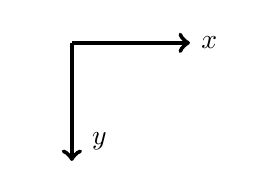
\begin{tikzpicture}
        \draw[->,ultra thick] (0,1.5)--(1.5,1.5) node[right]{$x$};
        \draw[->,ultra thick] (0,1.5)--(0.0,0.0) node[above]{\qquad$y$};
    \end{tikzpicture}}
    \qquad
    \begin{tabular}{c|>{\centering\arraybackslash}p{5mm}|>{\centering\arraybackslash}p{5mm}|>{\centering\arraybackslash}p{5mm}|}\cline{2-4}
                  & +1 & 0 & -1 \\\cline{2-4}
    $\frac{1}{6}$ & +1 & 0 & -1 \\\cline{2-4}
                  & +1 & 0 & -1 \\\cline{2-4}
    \end{tabular}
    \qquad
    \begin{tabular}{c|>{\centering\arraybackslash}p{5mm}|>{\centering\arraybackslash}p{5mm}|>{\centering\arraybackslash}p{5mm}|}\cline{2-4}
                  & +1 & +1 & +1 \\\cline{2-4}
    $\frac{1}{6}$ & \phantom{+}0 & \phantom{+}0 & \phantom{+}0 \\\cline{2-4}
                  & \laminus1 & \laminus1 & \laminus1 \\\cline{2-4}
    \end{tabular}
    \caption{Prewitt derivative operators}
    \vspace{-10mm}
    \label{fig:prewitt}
\end{figure}

\noindent\begin{minipage}{\textwidth}
\section{Edge detection}
\label{task:gradmag}
\begin{enumerate}
    \item Compute the \emph{magnitude} of the image gradient \begin{gather*}\left\|\nabla g\left(x,y\right)\right\| = \sqrt{g_x^2\left(x,y\right) + g_y^2\left(x,y\right)}\end{gather*} and include the resulting image into the notebook. \textbf{Hints:}
    \begin{enumerate}
        \item When working with objects of the type \texttt{numpy.ndarray} (e.g., images), mathematical operations are \emph{propagated} to the intensity values of the image. For example, if \texttt{img} is an image of the type \texttt{numpy.ndarray}, then the expression \texttt{img*2} yields an image with \emph{doubled} intensities (in comparison to \texttt{img}).
        \item The square root of an intensity value (or all values in an \texttt{numpy.ndarray} object) can be computed using the \texttt{sqrt} function (e.g., \texttt{sqrt(value)} or \texttt{sqrt(img)}).
    \end{enumerate}
    \item Quantitatively compare your result with the correct result image \texttt{data/\-lena\_\-prewitt\_\-gradmag.tiff}.
\end{enumerate}
\end{minipage}

\section{Sobel filter \bonustask}
\label{task:sobel}
Repeat Task~\ref{task:prewitt} using the \emph{Sobel} filter instead of the Prewitt filter:
\begin{enumerate}
    \item Compute the partial derivatives $g_x$ and $g_y$ by \emph{convolving} the image $g\left(x,y\right)$ with Sobel derivative operators (see Figure~\ref{fig:sobel}). To this end, implement the re-usable functions \texttt{sobel\_h} and \texttt{sobel\_v} analogously to \texttt{prewitt\_h} and \texttt{prewitt\_v}.
    \item Test your implementations for \texttt{sobel\_h} and \texttt{sobel\_v} by including images of the computed partial derivatives into your notebook (also include color legends).
    \item Quantitatively compare your results using \texttt{sobel\_h} and \texttt{sobel\_v} with the correct result images \texttt{data/lena\_sobel\_h.tiff} and \texttt{data/lena\_\-so\-bel\_\-v.tiff}, respectively.
\end{enumerate}
\begin{figure}[h!]
    \centering
    \raisebox{-0.8cm}{
    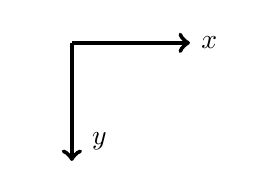
\begin{tikzpicture}
        \draw[->,ultra thick] (0,1.5)--(1.5,1.5) node[right]{$x$};
        \draw[->,ultra thick] (0,1.5)--(0.0,0.0) node[above]{\qquad$y$};
    \end{tikzpicture}}
    \qquad
    \begin{tabular}{c|>{\centering\arraybackslash}p{5mm}|>{\centering\arraybackslash}p{5mm}|>{\centering\arraybackslash}p{5mm}|}\cline{2-4}
                  & +1 & 0 & -1 \\\cline{2-4}
    $\frac{1}{8}$ & +2 & 0 & -2 \\\cline{2-4}
                  & +1 & 0 & -1 \\\cline{2-4}
    \end{tabular}
    \qquad
    \begin{tabular}{c|>{\centering\arraybackslash}p{5mm}|>{\centering\arraybackslash}p{5mm}|>{\centering\arraybackslash}p{5mm}|}\cline{2-4}
                  & +1 & +2 & +1 \\\cline{2-4}
    $\frac{1}{8}$ & \phantom{+}0 & \phantom{+}0 & \phantom{+}0 \\\cline{2-4}
                  & \laminus1 & \laminus2 & \laminus1 \\\cline{2-4}
    \end{tabular}
    \caption{Sobel derivative operators}
    \label{fig:sobel}
\end{figure}

\end{document}
